In einem Spiel werden zwei Würfel geworfen und als Gewinn
der grösste gemeinsame Teiler der Augenzahlen ausbezahlt.
\begin{teilaufgaben}
\item
Welchen Gewinn erwarten Sie?
\item
Welche Varianz hat der Gewinn?
\end{teilaufgaben}

\thema{Laplace-Experiment}
\thema{Erwartungswert}
\thema{Varianz}

\begin{loesung}
\begin{figure}
\centering
\includeagraphics[]{graph-1.pdf}
\caption{Histogramm der Gewinne in Aufgabe~\ref{40000023}
\label{40000023:histogram}}
\end{figure}
Sei $X$ die Zufallsvariable des Gewinns.
Es führt wohl nichts daran vorbei, alle möglichen Gewinne aufzulisten.
Diese sind in einer quadratischen Tabelle mit den Augenzahlebn der beiden 
Würfel als Koordinaten wie folgt zusammengefasst:
%\[
%\begin{tabular}{|cccccc|}
%\hline
%1&1&1&1&1&1\\
%1&2&1&2&1&2\\
%1&1&3&1&1&3\\
%1&2&1&4&1&2\\
%1&1&1&1&5&1\\
%1&2&3&2&1&6\\
%\hline
%\end{tabular}
%\]
\begin{center}
\def\feld#1#2#3{
	\node at ({(#1-0.5)*\h},{(6.5-(#2))*\h}) {\strut$#3\mathstrut$};
}
\def\h{0.6}
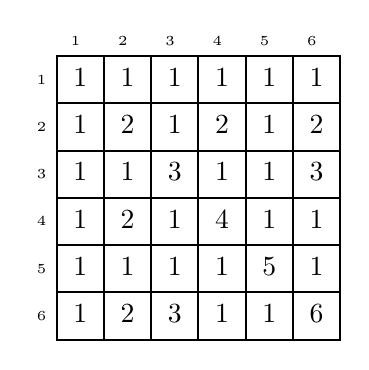
\begin{tikzpicture}[>=latex,thick]
\draw (0,0) rectangle ({6*\h},{6*\h});
\foreach \x in {1,2,3,4,5}{
	\draw ({\x*\h},0) -- ++(0,{6*\h});
	\draw (0,{\x*\h}) -- ++({6*\h},0);
}

\foreach \k in {1,...,6}{
	\node at ({(\k-0.6)*\h},{6*\h}) [above] {\tiny $\k$};
	\node at (0,{(6.5-\k)*\h}) [left] {\tiny $\k$};
}

\feld{1}{1}{1} \feld{1}{2}{1} \feld{1}{3}{1} \feld{1}{4}{1} \feld{1}{5}{1} \feld{1}{6}{1}
\feld{2}{1}{1} \feld{2}{2}{2} \feld{2}{3}{1} \feld{2}{4}{2} \feld{2}{5}{1} \feld{2}{6}{2}
\feld{3}{1}{1} \feld{3}{2}{1} \feld{3}{3}{3} \feld{3}{4}{1} \feld{3}{5}{1} \feld{3}{6}{3}
\feld{4}{1}{1} \feld{4}{2}{2} \feld{4}{3}{1} \feld{4}{4}{4} \feld{4}{5}{1} \feld{4}{6}{1}
\feld{5}{1}{1} \feld{5}{2}{1} \feld{5}{3}{1} \feld{5}{4}{1} \feld{5}{5}{5} \feld{5}{6}{1}
\feld{6}{1}{1} \feld{6}{2}{2} \feld{6}{3}{3} \feld{6}{4}{1} \feld{6}{5}{1} \feld{6}{6}{6}
\end{tikzpicture}
\end{center}
Daraus kann man abzählen, dass die Werte 1 bis 6 folgende
Wahrscheinlichkeiten haben, ein Histogram der Gewinne ist in 
Abbildung~\ref{40000023:histogram} dargestellt.
\[
\setlength\extrarowheight{3pt}
\begin{tabular}{>{$}c<{$}|>{$}c<{$}}
\text{Wert}&\text{Wahrscheinlichkeit}\\
\hline
1& \frac{23}{36} \\
2& \frac{ 7}{36} \\
3& \frac{ 3}{36} \\
4& \frac{ 1}{36} \\
5& \frac{ 1}{36} \\
6& \frac{ 1}{36} 
\end{tabular}
\]
Daraus kann man die benötigten Erwartungswerte ermitteln.
\begin{teilaufgaben}
\item
Der Erwartungswert des Gewinns ist
\begin{align*}
E(X)&=
1\cdot\frac{23}{36}+
2\cdot\frac{7}{36}+
3\cdot\frac{3}{36}+
4\cdot\frac{1}{36}+
5\cdot\frac{1}{36}+
6\cdot\frac{1}{36}
\\
&=\frac{23 + 2\cdot 7 + 3\cdot 3+4\cdot 1+5\cdot 1+6\cdot 1}{36}\\
&=\frac{23 + 14 + 9 + 4+5+6}{36}
=\frac{61}{36}=1.69444.
\end{align*}
\item
Für die Varianz brauchen wir zunächst den Erwartungswert $E(X^2)$:
\begin{align*}
E(X^2)&=
1^2\cdot\frac{23}{36}+
2^2\cdot\frac{7}{36}+
3^2\cdot\frac{3}{36}+
4^2\cdot\frac{1}{36}+
5^2\cdot\frac{1}{36}+
6^2\cdot\frac{1}{36}
\\
&=\frac{23 + 4\cdot 7 + 9\cdot 3+16\cdot 1+25\cdot 1+36\cdot 1}{36}\\
&=\frac{23 + 28 + 27 + 16+25+36}{36}
=\frac{155}{36}.
\end{align*}
Jetzt kann man daraus die Varianz bestimmen:
\begin{align*}
\operatorname{var}(X)
&=
E(X^2)-E(X)^2
=
\frac{155}{36}-\biggl(\frac{61}{36}\biggr)^2
=
\frac{155\cdot 36-61^2}{36^2}=\frac{1859}{1296}\simeq 1.4344.
\qedhere
\end{align*}
\end{teilaufgaben}
\end{loesung}

